\documentclass[a4paper, 11pt, titlepage]{jsarticle}
\usepackage[dvipdfmx]{graphicx}
\usepackage{listings}
\usepackage{amsmath}
\usepackage{url}


\title{知能情報実験III(データマイニング班)\\指紋認証を用いたCNNの手法についての模索}
\author{\textbf{185710A 金城海斗}\\
\textbf{185714C 石橋竜弥}\\
 \textbf{185745C 上間翔}\\
 \textbf{185752F 新垣裕二}\\
 \textbf{185763B 草薙幸菜}}
\date{提出日:2021年2月x日}
\begin{document}
\maketitle
\tableofcontents
\clearpage


\section{はじめに}
データマイニングとはデータの中に埋め込まれている有用な知識を発掘することである。別の言い方では、データマイニングは、より良い意思決定をするために履歴データをうまく使って一般的な規則性を発見しよとする研究分野である。今回私たちのグループ3では、機会学習の基本的な考え方を実装、体験を通して学んだ。そしてその応用として、既存に存在する指紋データを使った指紋認証のプログラムの分析から、畳み込みニューラルネットワークの手法についての模索、改善を行い、結果の精度向上を目指し、考察したことについて述べていく。

\subsection{Convolutional Neural Network:CNN}
Convolutional Neural Network (これよりCNNと呼ぶ)は畳み込みニューラルネットワークという意味であり、機械学習で画像の深層学習といえばCNNであるというほどよく使われている識別手法である。これは、ニューラルネットワークに畳み込みという操作を導入したものである。CNNについて、簡単な手順を記述する。まず手順1として、\textbf{画像から特徴を抽出}する。フィルタを使い、入力層データの中で位置を変えながらスキャンした部分のデータと、フィルター自身の持つデータとの差異を畳み込みの結果として畳み込みそうに書き込んだものを特徴量といい、入力層の全データをスキャンしてできた畳み込み結果の値の集まりを特徴マップという。複数のフィルタを用意することで、入力層のデータ特徴を捉えやすくしている。下の図は用意した複数フィルタのうち、一つが完全に入力層のデータの一部と同じであることを示す。

\begin{figure}[h]
  \centering
  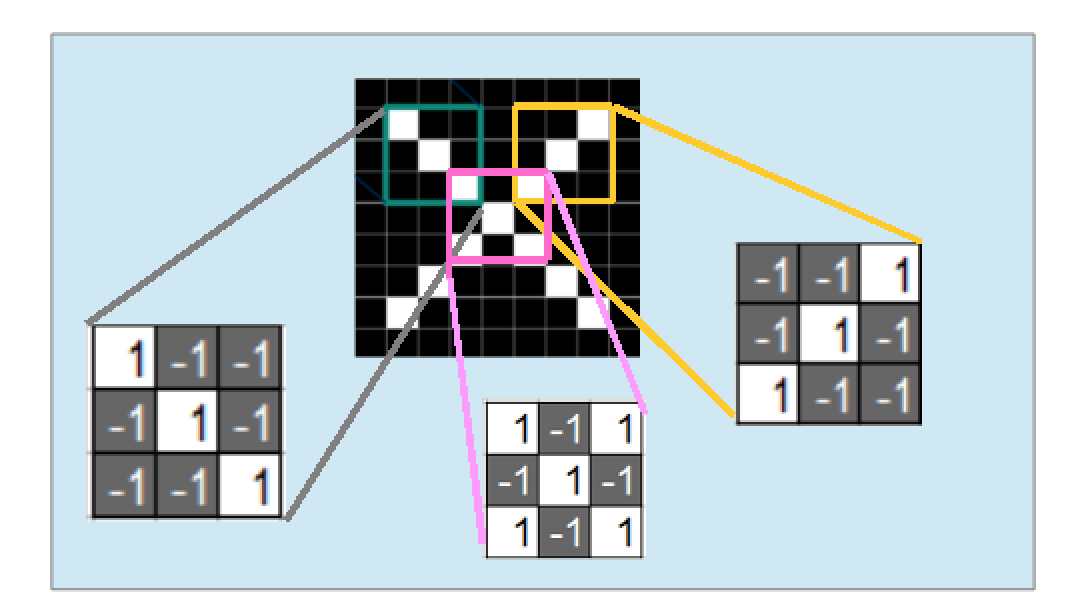
\includegraphics[scale=0.4]{cnn1.png}
  \caption{CNN解説手順1}
  \label{cnn}
\end{figure}


手順2として、\textbf{画像を畳み込み}する。入力層のデータをフィルターのデータとピクセル毎に比較することで、畳み込み層にその類似度(特徴量)を書き込む。下記の図はフィルタを利用して特徴量を抽出し、特徴マップを作成した例である。

\begin{figure}[h]
  \centering
  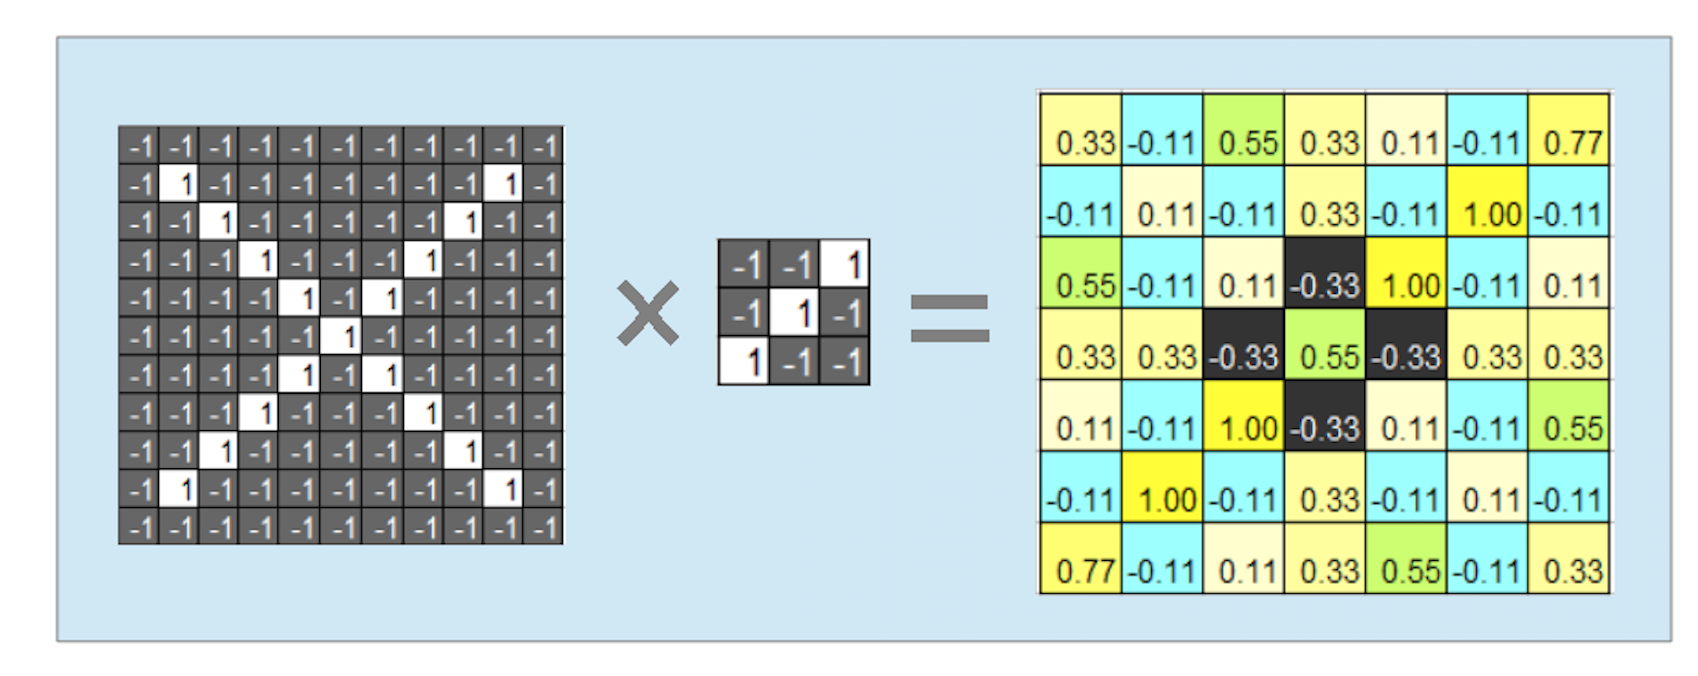
\includegraphics[scale=0.3]{cnn2.png}
  \caption{CNN解説手順2}
  \label{cnn}
\end{figure}

手順3として、\textbf{画像をプーリング}する。畳み込みの層の情報はプーリング層で集約する。出力に関しては、プーリング層のユニット全てと全結合し、計算結果を利用して、フィルタ、重み、バイアスを更新していく。

\begin{figure}[h]
  \centering
  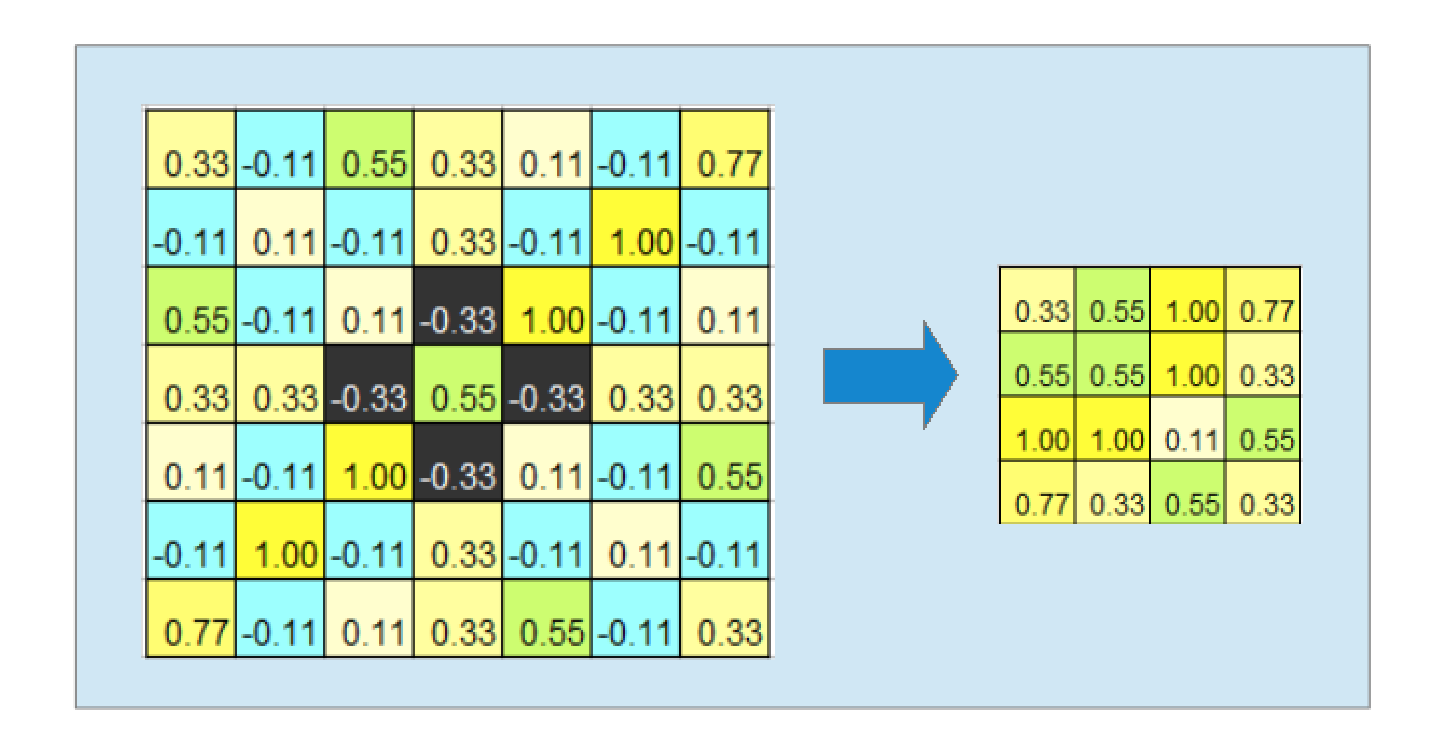
\includegraphics[scale=0.3]{cnn3.png}
  \caption{CNN解説手順3}
  \label{cnn}
\end{figure}


\subsection{テーマ指紋認証とは}
本グループでは、授業の中でデータマイニングについて学び、それらの応用実験として、画像認識について分析しようと考えた。そして、データマイニングを行う識別手としてCNNに目をつけ、データの分類ラベルがはっきりしており、複雑である指紋認証の分析、精度改善を行うこととなった。CNNは畳み込み処理を利用したニューラルネットワークであり、どのくらい畳み込み処理を行うのか、どのくらいニューラルネットワークを深くするのかは定義されていない。


\section{実験方法}


\subsection{実験目的}



\subsection{データセット構築}
Kaggleより、指紋のデータセットを利用している。\url{https://www.kaggle.com/ruizgara/socofing}

\subsection{モデル選定}
アルゴリズムは序章で述べたとおり、CNNを利用しており、以下のコードを参考にしている。\url{https://www.kaggle.com/brianzz/subjectid-finger-cnnrecognizer}\\
本アルゴリズムの運用において、指紋認証の正答率が十分に高い点、可読性に優れており改善手法を模索しやすい点に特に優れているため使用することにした。

\subsection{パラメータ調整}
CNNのパラメータ調整では、epoch数・画像データ数・batchsizeや活性化関数であるLeakyReLUを変更していった。


%\newpage
\section{実験結果}
%事実として得られた結果を示そう。
%なお、以下の点に留意すること。

実験結果として、以下の結果が得られた。%ここの条件(batch_sizeとかmodelの中身とか)の補足をお願いします。
%epoch10の値の共通項がコピペ事故起こしてそうですが大丈夫ですか?

\subsection{エポック数を1から30までに変化}
\begin{table}[htb]
  \begin{tabular}{|l|c|c|}
    \hline
    epoch & subjectID accracy & fingerNum accracy \\ \hline
    1 & 01.5333333052694798 \% & 63.01666498184204 \%  \\ \hline
    3 & 61.283332109451294 \% & 89.48333263397217 \% \\ \hline
    5 & 96.35000228881836 \% & 98.15000295639038 \%  \\ \hline
    10 & 99.71666932106018 \% & 99.71666932106018 \%  \\ \hline
    20 & 99.73333477973938 \% & 99.88333582878113 \%  \\ \hline
    30 & 99.73333477973938 \% & 99.90000128746033 \% \\ \hline
  \end{tabular}
\end{table}

\subsection{epochを20に固定し、batch\_sizeを変更}%アンダーバーは関数記号?エラーの元。ただの記号にするためのバックスラッシュが必要
\begin{table}[htb]
  \begin{tabular}{|l|c|c|}
    \hline
    batch\_size & subjectID accuracy & fingerNum accuracy  \\ \hline
    32 & 99.73333477973938 \% & 99.90000128746033 \% \\ \hline
    64 & 99.73333477973938 \% & 99.88333582878113 \% \\ \hline
    128 & 99.71666932106018 \% & 99.88333582878113 \% \\ \hline
  \end{tabular}
\end{table}

%ここの条件(batch_sizeとかepochとか)の補足をお願いします。
\subsection{活性化関数に変更}
\begin{table}[htb]
  \begin{tabular}{|l|c|c|}
    \hline
    活性化関数 & subjectID accracy & fingerNum accracy \\ \hline
    LeakyReLU (alpha=-0.5) & 99.43333268165588 \% & 99.88333582878113 \% \\ \hline
    LeakyReLU (alpha=0.3) & 99.71666932106018 \% & 99.73333477973938 \% \\ \hline
    LeakyReLU (alpha=0.5) & 99.6999979019165 \% & 99.6333360671997 \% \\ \hline
    sigmoid & 99.73333477973938 \% & 99.86666440963745 \% \\ \hline
    tanh & 99.73333477973938 \% & 99.88333582878113 \% \\ \hline
  \end{tabular}
\end{table}

\clearpage


\section{考察}
初めに、元のサンプルコードの条件はエポック数20のバッチサイズ64、活性化関数は中間層でReLU関数を用いて、出力層に対してsoftmax関数を用いている。結論から言うと、どの条件下においても大きな変化は見られなかった。精度を向上させることができた条件は、エポック数を20から30に増やすこと、バッチサイズを64から32に変更することの2つであった。また、両者とも精度が上がったのは fingerNum accracy、つまりどの指であるかの識別するものであった。この原因と、その他の条件において精度が上昇しなかった原因について考える。

初めに、fingerNum accracyのみ精度が向上したことについて考える。まず、エポック数とは学習する世代のことであり、これを多くしていくことで細かい識別が可能になる。直感的に考えれば、10本のうちどの指かを識別するよりも、600人のうち誰の指紋であるかを識別する方が難しいはずであるが、このことからfingerNum accracyの方が細かい識別が必要になると考える。

次に、活性化関数を変更した場合について考える。今回は画像の識別であるため、活性化関数も多くの値を表現できるものが良いと考えた。0と1だけで識別するのと、1から100までを用いて識別するのは後者の方がより細かいものを表現できるはずである。実際、元のサンプルコードは正の値はそのまま使用するReLU関数を用いていた。そこで、負の値も一定の割合で使用するLeakyReLU関数を用いたが結果は精度がやや落ちる程度だった。また、sigmoid関数とtanh関数も用いた。これらは入力された値を、0から1、-1から1の実数にする関数である。これまでの考えだと精度は下がると予測したが、LeakyReLU関数を用いた結果とあまり大差はなかった。これらのことを見ると活性化関数に精度との相関が見られない。活性化関数の他に精度をあげている要因があると考えられる。今回の実験では最適化関数について変更を行っていため、最適化関数に原因があるのではないかと考える。

以上より、エポック数による精度の向上はやや見られたが、活性化関数が識別にどのような効果をもたらしているのかは読み取ることができなかった。

%追加する時のtemplate
\begin{table}[htb]
  \begin{tabular}{|l|c|c|}
    \hline
    hogehoge & subjectID accuracy & fingerNum accuracy  \\ \hline
    hoge & hoge \% & hoge \% \\ \hline
    hoge & hoge \% & hoge \% \\ \hline
  \end{tabular}
\end{table}

\section{意図していた実験計画との違い}
当初予定していた実験計画は以下の通りとなる。
\begin{itemize}
\item	6週目(11/17):テーマ決め、データセット探し、あと色々
\item	7週目(11/24):特徴ベクトルの抽出とかコード探して理解したりとか
\item	8週目(12/1)  :画像認識をコードに落とし込む
\item	9週目(12/8)  :実験開始?出来上がったコードを動かす段階?
\item	10週目(12/15):コードや特徴ベクトルの調整1
\item	11週目(12/22):
\item	12週目(1/5)  :
\item	13週目(1/12):改善実験?
\item	14週目(1/19):
\item	15週目(1/26):レポート・プレゼン資料作成
\item	期末テスト日(2/2):最終発表
\end{itemize}
上記の予定は11/17日に作成されたもの。これ以降に追加された締め切り予定に、
\begin{itemize}
\item	15週目(1/26):レポート初期版の提出日
\item	(2/16):Github公開
\end{itemize}
がある。

実際の進捗の経過をまとめると、下記の通りとなる。
\begin{itemize}
\item	6週目(11/17):テーマ決定(画像認証/fingerprint)・データセット探し、画像認証に対しての学習
\item	7週目(11/24):指紋の特徴量の分析、CNNの画像認証コードの検索
\item	8週目(12/1)  :参考するCNNコードの決定、コードの内容の分析・実行%私だけPython消してました
\item	9週目(12/8)  :コードの内容の分析・実行2nd
\item	10週目(12/15):コードの内容の分析3rd・amaneによる実行開始・実験目的の草案
\item	11週目(12/22):コードの内容の分析4th・実行2nd。またamaneで画像データの出力は難しいと判断。来年度に向けたの引継ぎ
\item	12週目(1/5)  :コードの内容の分析5th・epoch数を変えた大規模実験・Python/Keras環境の統一
\item	13週目(1/12):コードの内容の分析6th・batch\_sizeやLeakyReLUを変更した実験
\item	14週目(1/19):レポートの作成・amaneによる実験
\item	15週目(1/26):
\item	期末テスト日(2/2):
\end{itemize}



\section{まとめ}
データマイニング班の達成目標を振り返り、選んだテーマに対する機械学習の適用を通して得られた知見や学んだことをまとめよう。
また今後やるべきことや後進に伝えたいこと等あれば自由に述べよう。

\begin{thebibliography}{n}
  \bibitem{cnn} CNN解説, \\
  \url{https://udemy.benesse.co.jp/data-science/ai/convolution-neural-network.html}, 2021/01/026.
  \bibitem{dataset}指紋データセット, 
  \url{https://www.kaggle.com/ruizgara/socofing}
  \bibitem{algorithm}アルゴリズム, \url{https://www.kaggle.com/ruizgara/socofing}
  \bibitem{}
\end{thebibliography}

\end{document}
